%----------------------------------------
% Write your notes here
%----------------------------------------

\section{Introduction}
Framework for Models:
\begin{itemize}
  \item Specify outcome and predictors
  \item Actually a difficult part (usually handed to you)
  \item Define loss function
  \item How close model predicts compared with observed data
  \item Develop algorithm to find the best model
  \item Mnimize loss function (searching across all possible methods)
  \item Assess model performance + results
\end{itemize}

\vspace{10mm}

Regressions:

\begin{equation}
Outcomes: \lbrace {y_i} \rbrace^N_{i=1}
\end{equation}

\begin{equation}
Predictors: \lbrace {x_i} \rbrace^N_{i=1} \hspace{5mm}  (Input/Features)
\end{equation}

\vspace{5mm}
X can be a vector of multiple dimensions, or features

\pagebreak

Figure \ref{fig:example_figure} k-dimensional vector

\begin{figure}[ht]
  \begin{center}
    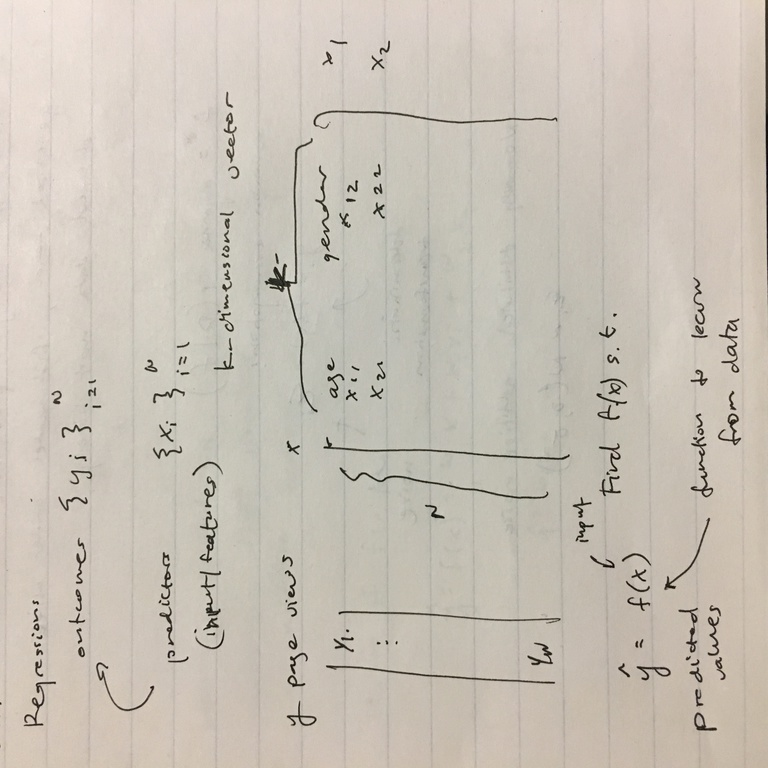
\includegraphics[width=.9\textwidth,angle=270]{figures/IMG_6640.JPG}
    \caption{
      Aim to learn coefficients for vector x to predict y.}
    \label{fig:example_figure}
  \end{center}
\end{figure}

\pagebreak

Figure \ref{fig:example_figure2} Define a loss function to minimize

\begin{figure}[ht]
  \begin{center}
    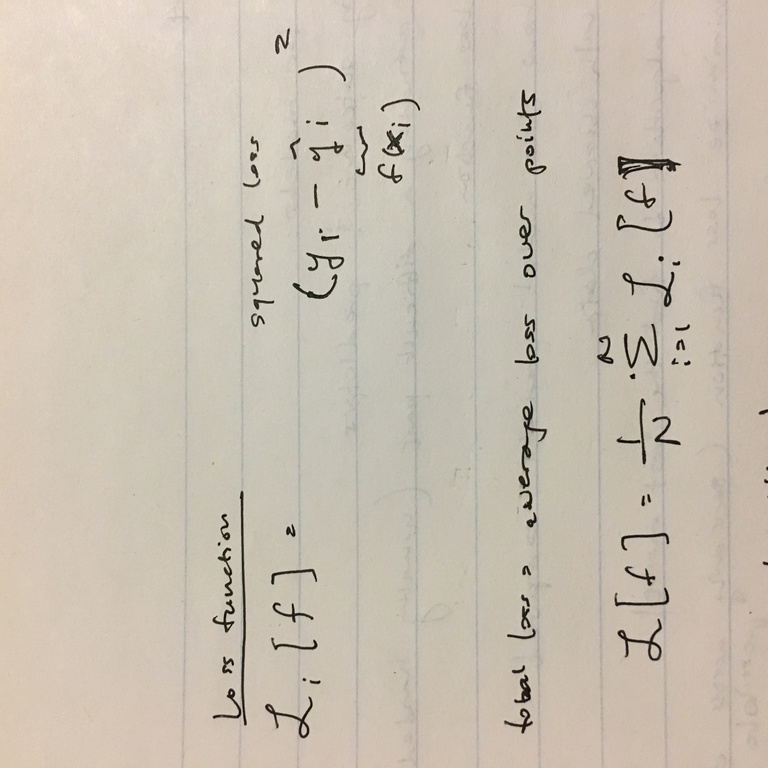
\includegraphics[width=.9\textwidth,angle=270]{figures/IMG_6641.JPG}
    \caption{
      Minimizing loss function allows to find coefficients with least error.}
    \label{fig:example_figure2}
  \end{center}
\end{figure}

\pagebreak

Figure \ref{fig:example_figure3} Maximum Likelihood
\begin{figure}[ht]
  \begin{center}
    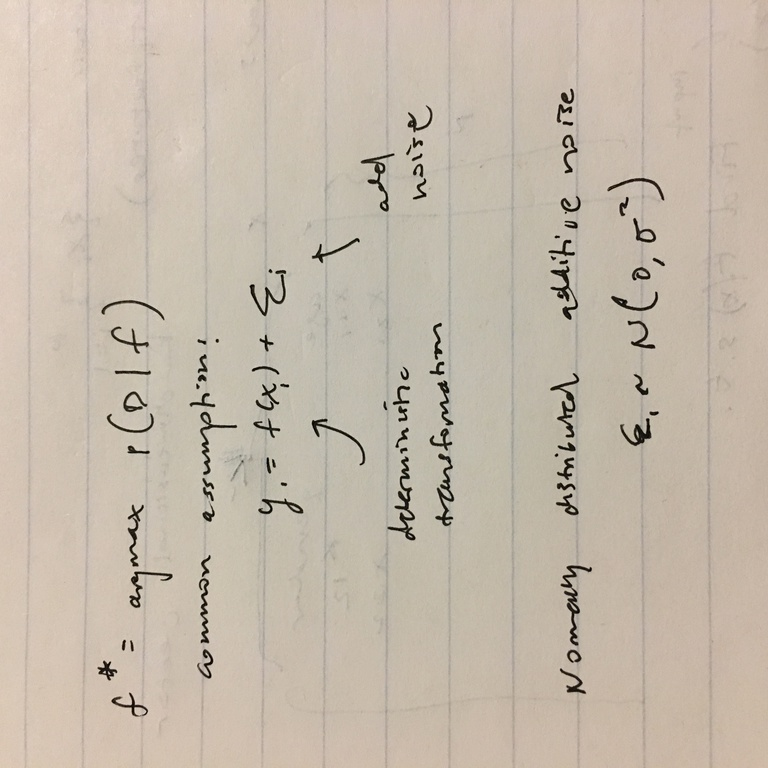
\includegraphics[width=.9\textwidth,angle=270]{figures/IMG_6642.JPG}
    \caption{
      Assume some family of probabilistic models generated the data - we find the model
      under which observed data most likely}
    \label{fig:example_figure3}
  \end{center}
\end{figure}

\pagebreak

Figure \ref{fig:example_figure4} Maximizing given error

\begin{figure}[ht]
  \begin{center}
    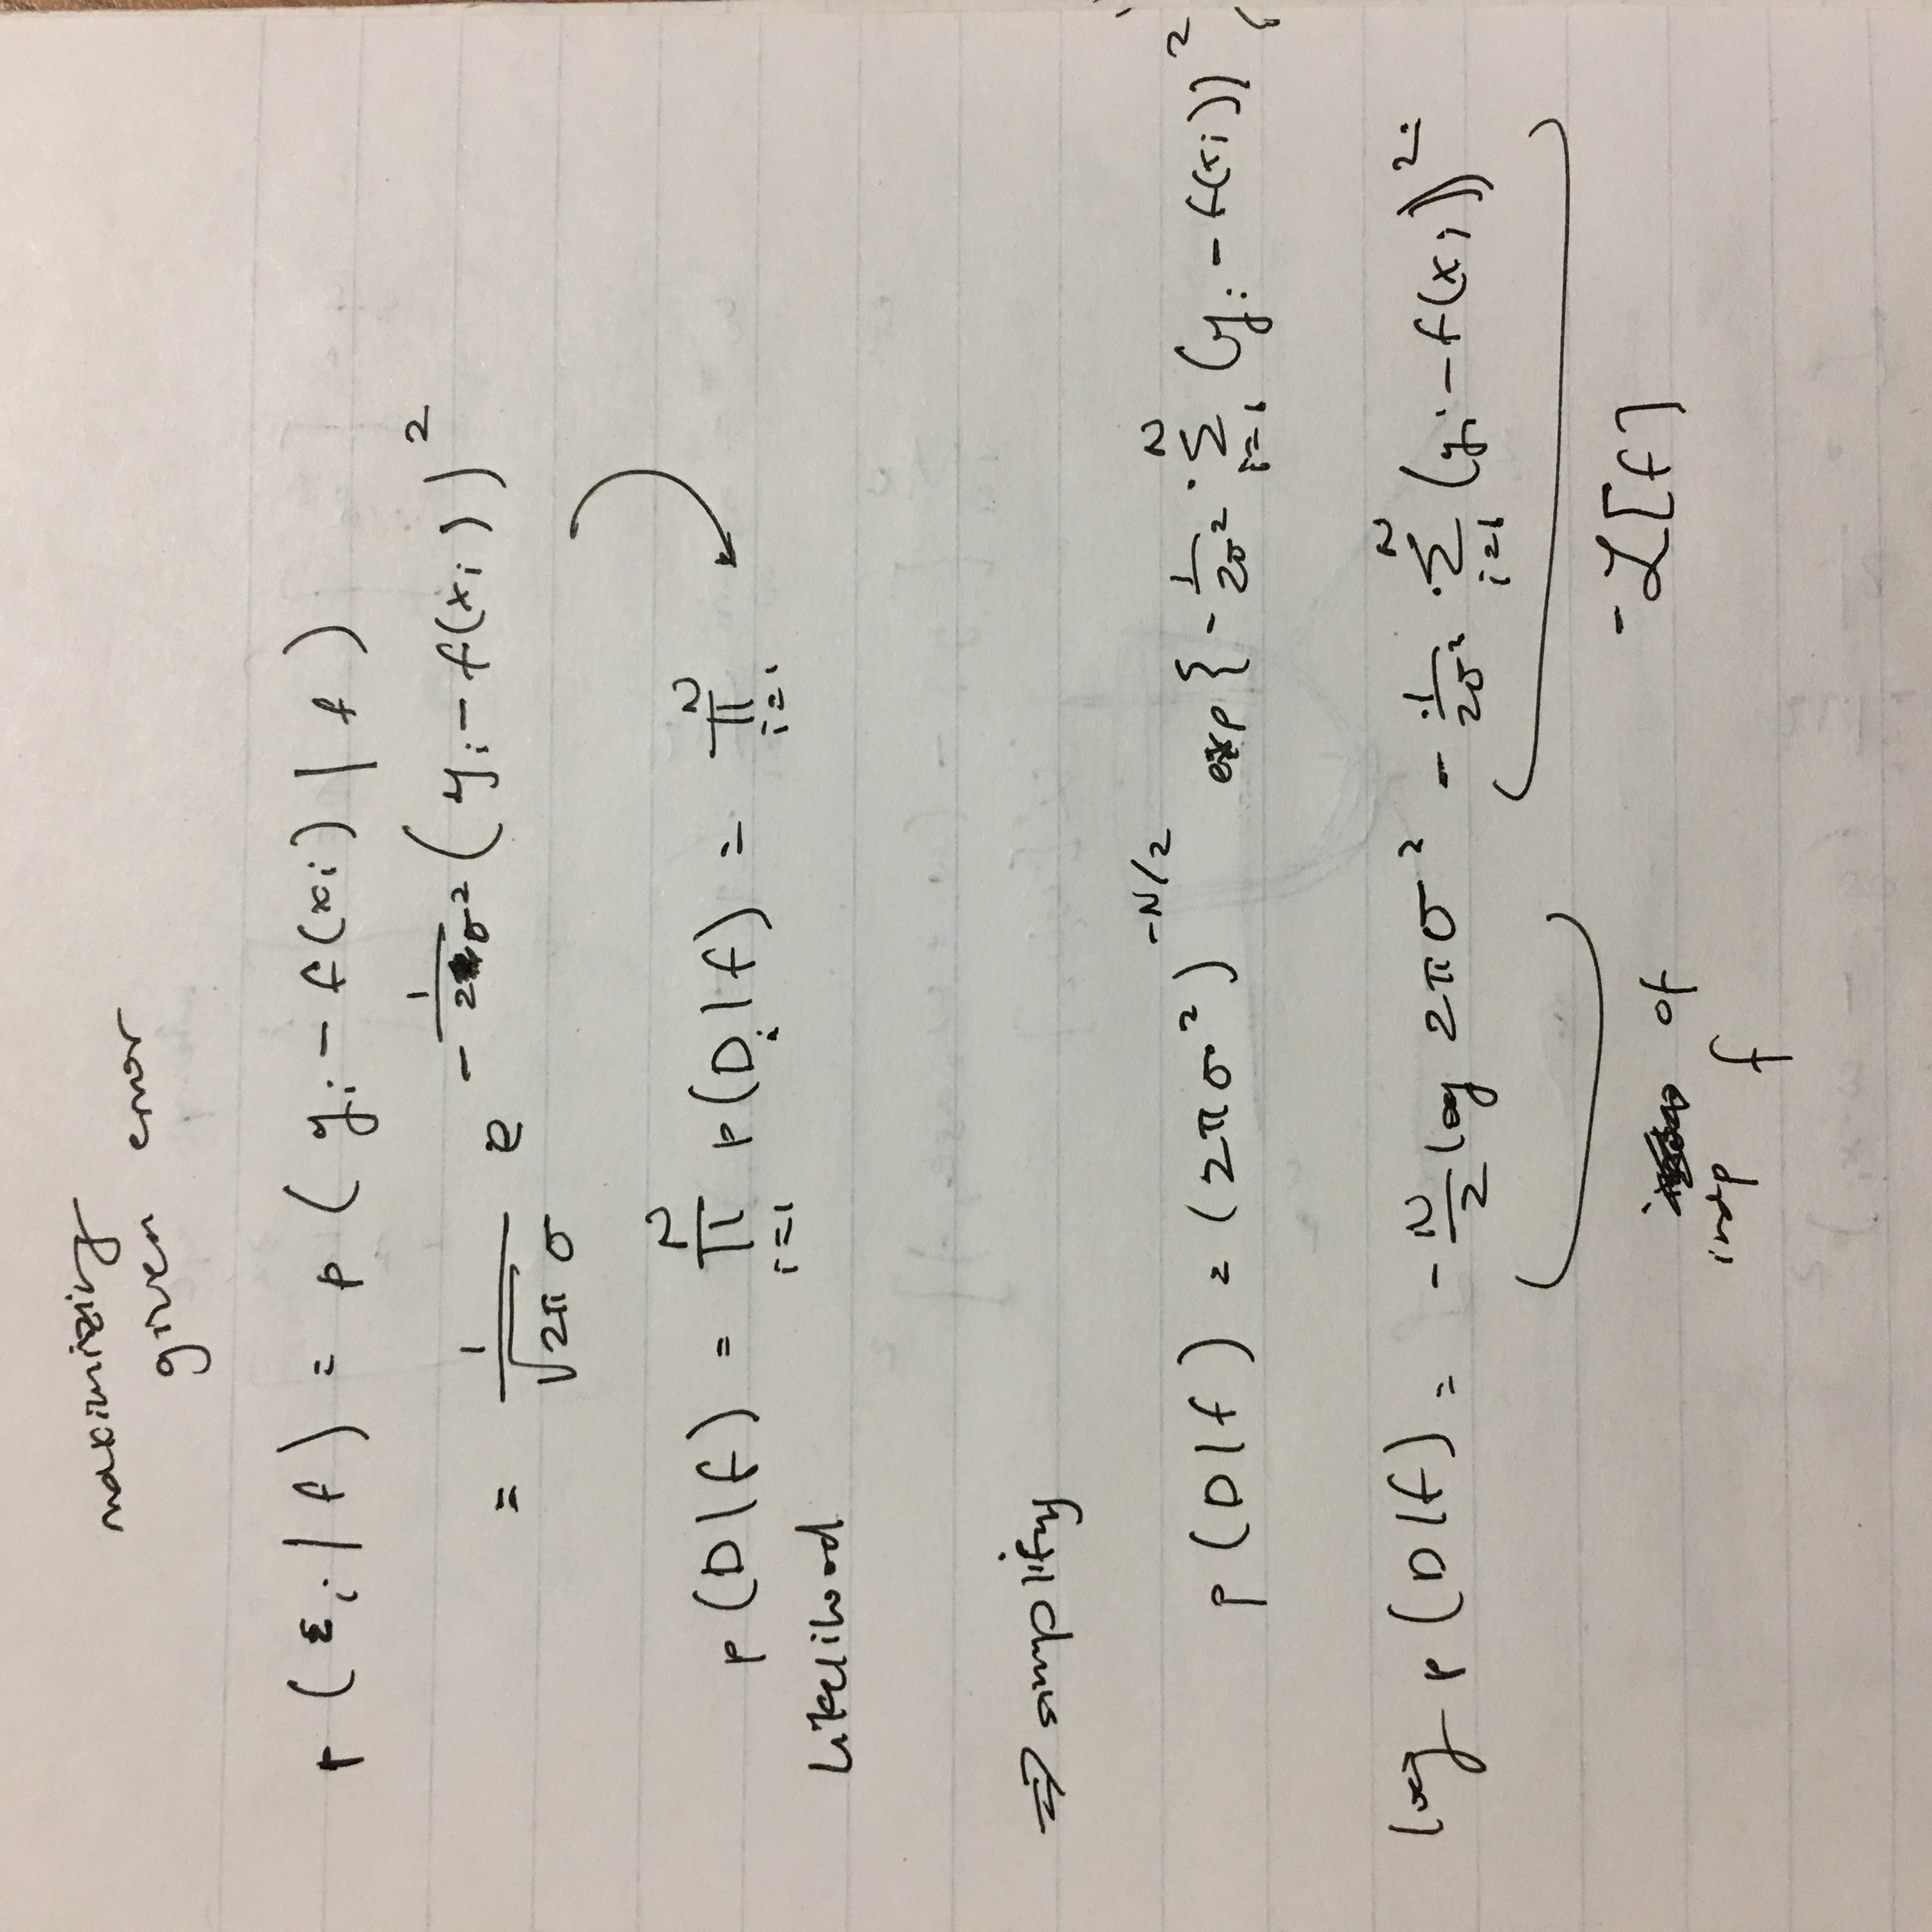
\includegraphics[width=.9\textwidth,angle=270]{figures/4.jpg}
    \caption{
      Minimizing squared loss is equivalent to maximizing (log) likelihood, assuming additive
      Gaussian noise.}
    \label{fig:example_figure4}
  \end{center}
\end{figure}

\pagebreak

Figure \ref{fig:example_figure5} 

\begin{figure}[ht]
  \begin{center}
    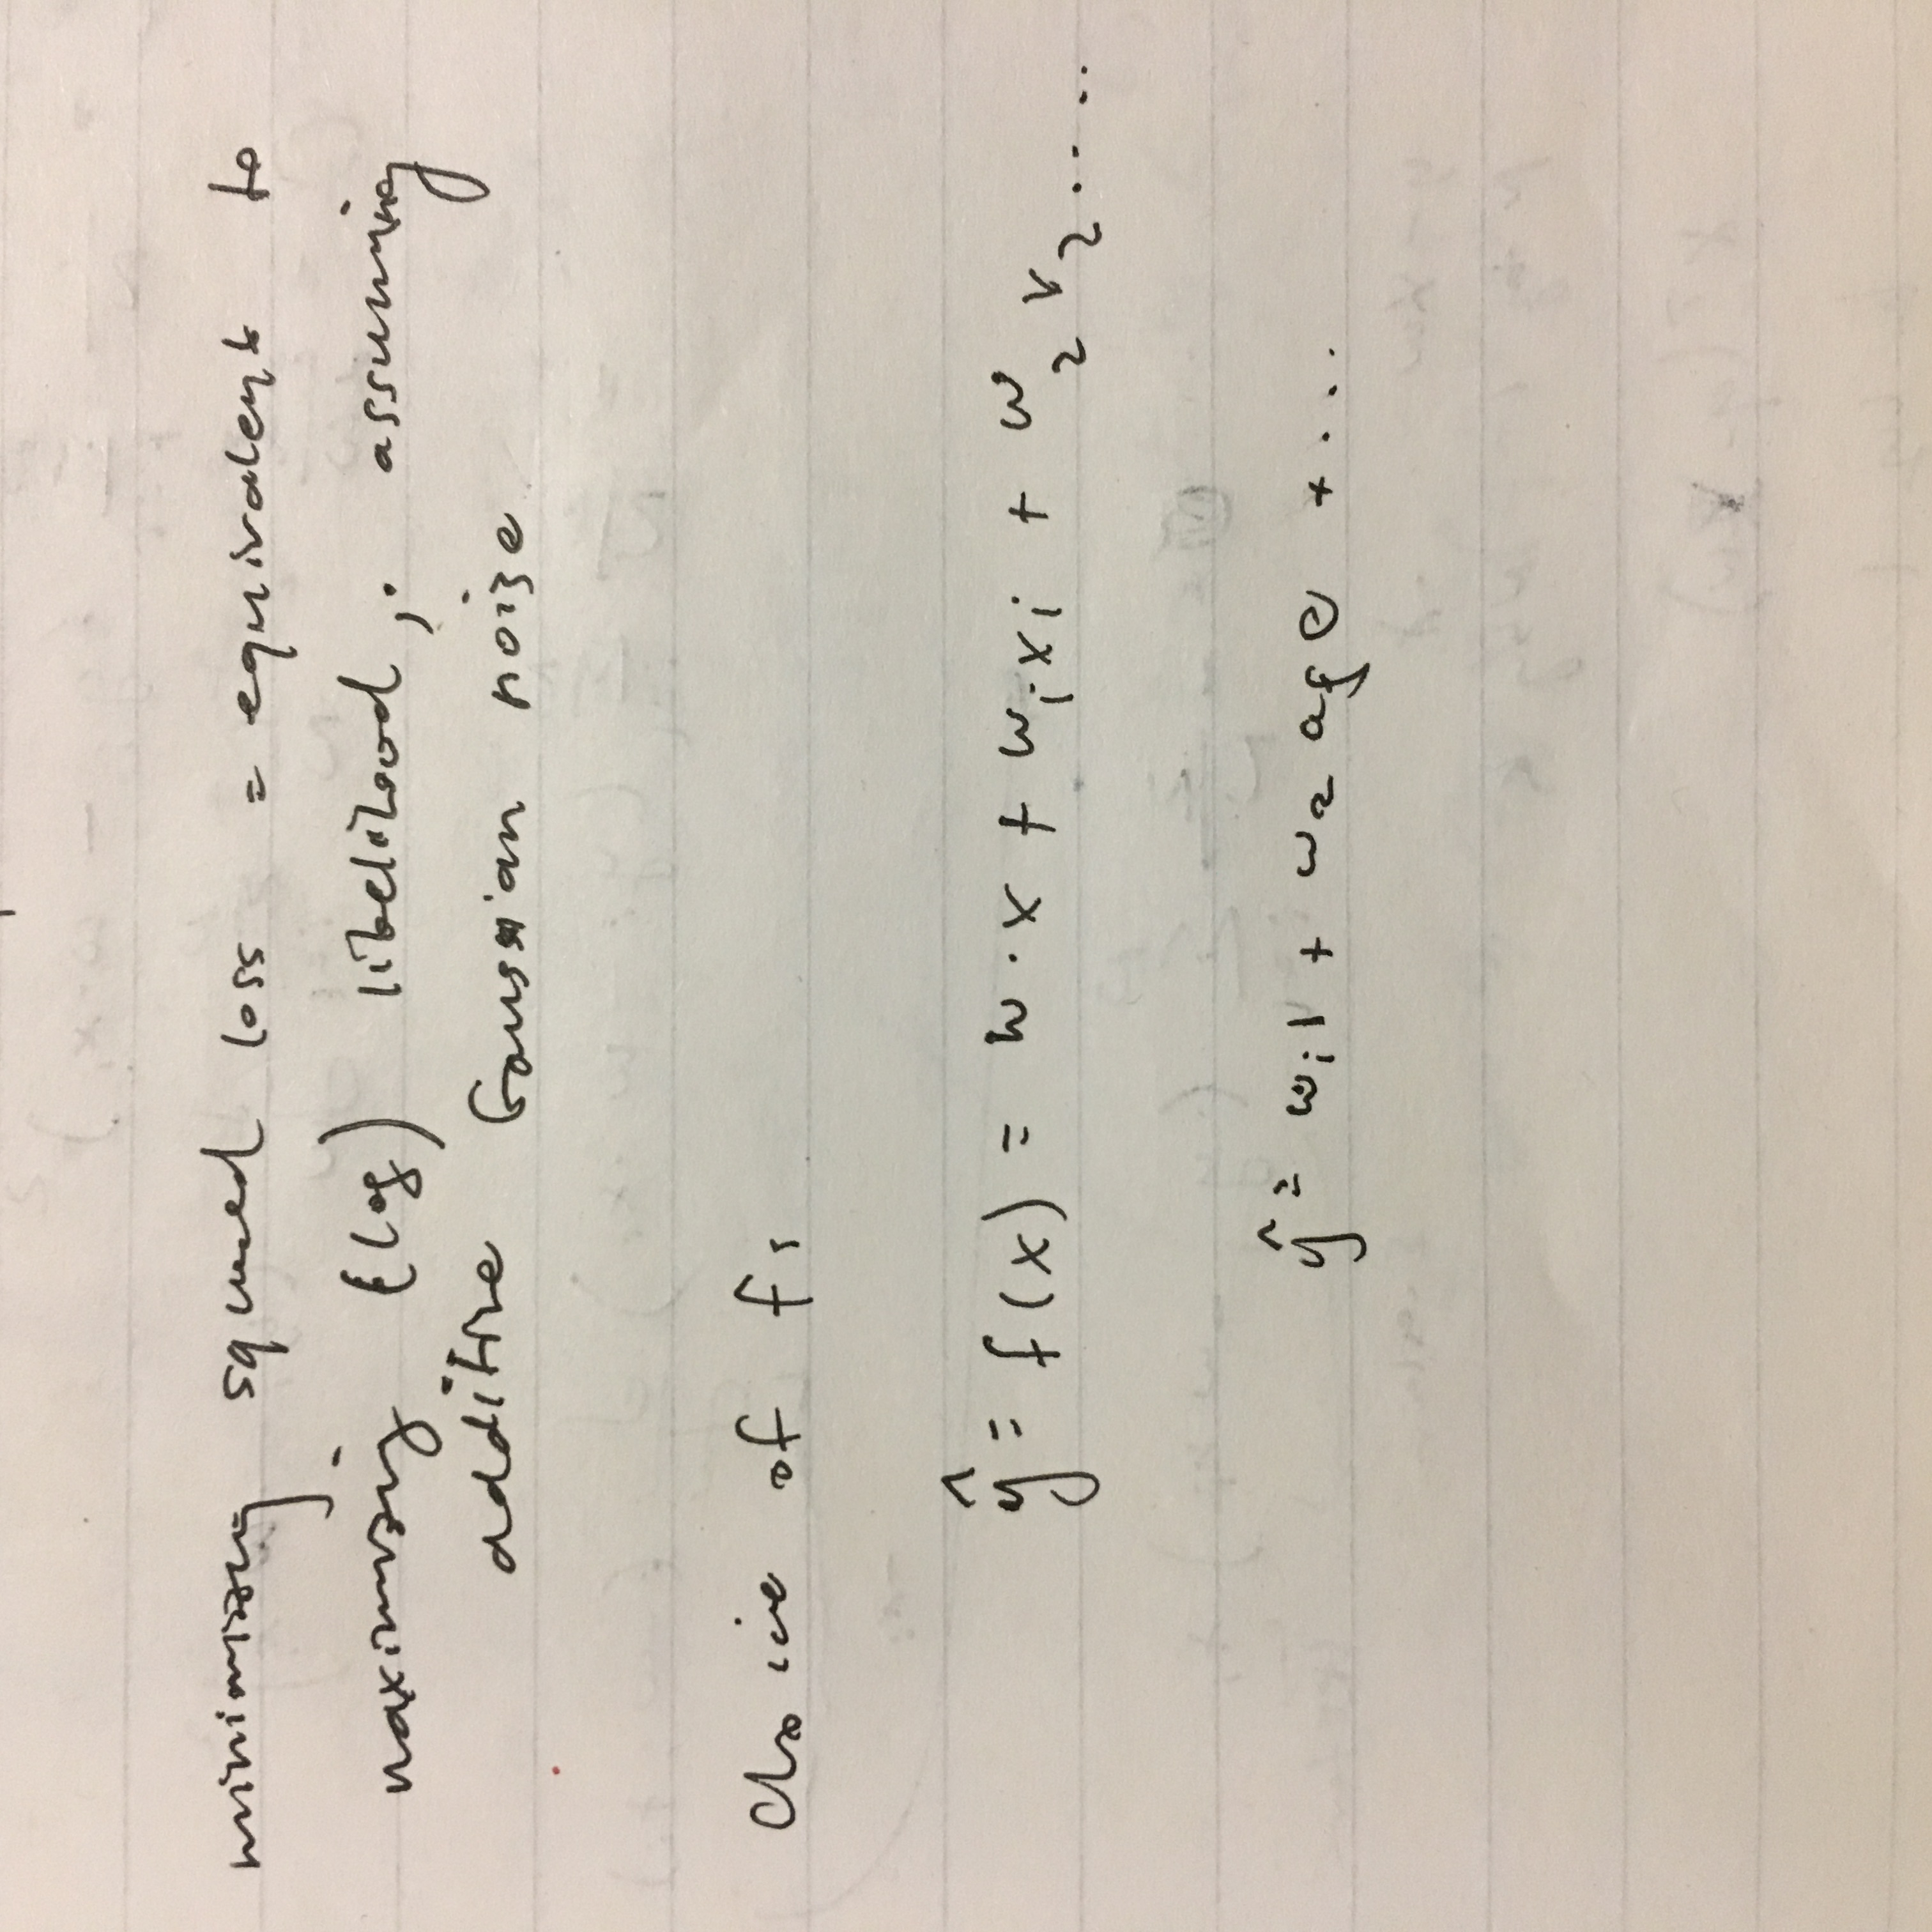
\includegraphics[width=.9\textwidth,angle=270]{figures/5.jpg}
    \caption{
    	Minimizing squared loss is equivalent to maximizing (log) likelihood, assuming 					additive Gaussian noise.
      }
    \label{fig:example_figure5}
  \end{center}
\end{figure}

\pagebreak

Figure \ref{fig:example_figure6} Two Dimensional Representation of Loss Function

\begin{figure}[ht]
  \begin{center}
    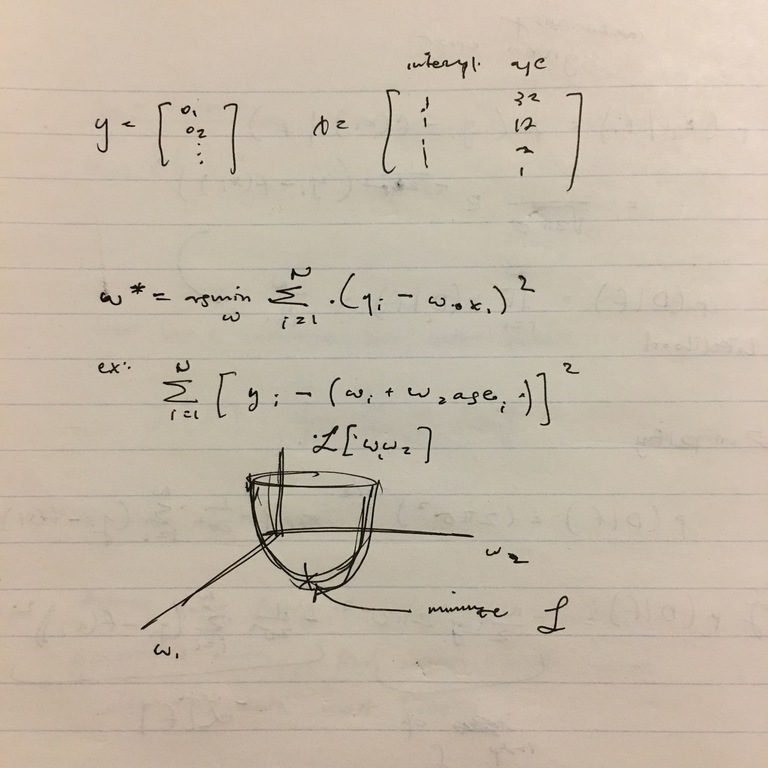
\includegraphics[width=.9\textwidth]{figures/FullSizeRender.jpg}
    \caption{
      If we are working with two dimensions(labels), easier to visualize minimizing L to find
      coefficients with least loss}
    \label{fig:example_figure6}
  \end{center}
\end{figure}

\pagebreak

Figure \ref{fig:example_figure7} Mathematical derivation
\begin{figure}[ht]
  \begin{center}
    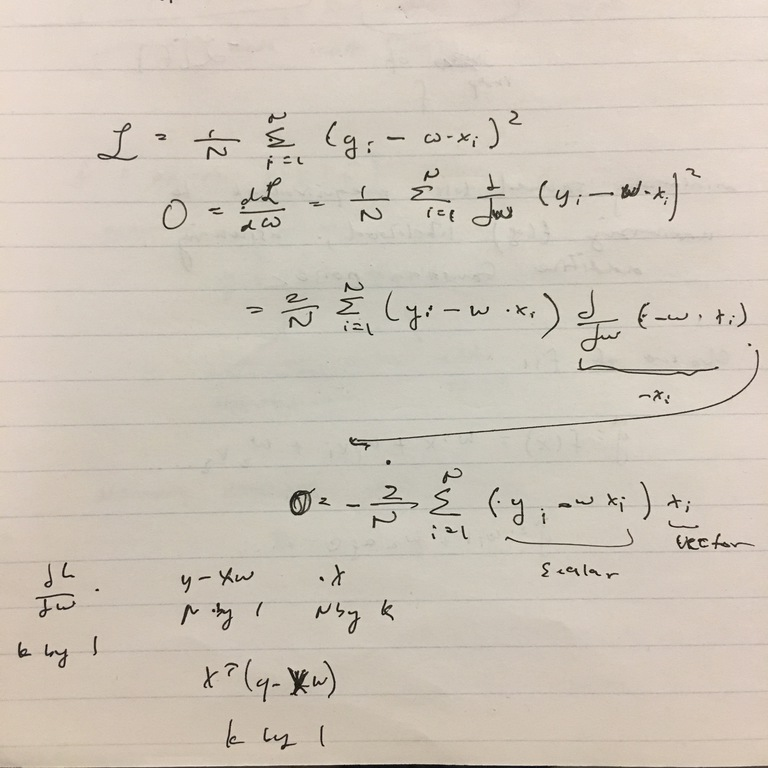
\includegraphics[width=.9\textwidth]{figures/FullSizeRender_2.jpg}
    \caption{
      Take derivative of loss function (averaged over all values) and set to 0 to solve for our
      vector of coefficients.}
    \label{fig:example_figure7}
  \end{center}
\end{figure}

\pagebreak

Figure \ref{fig:example_figure8} Converting to matrix operations

\begin{figure}[ht]
  \begin{center}
    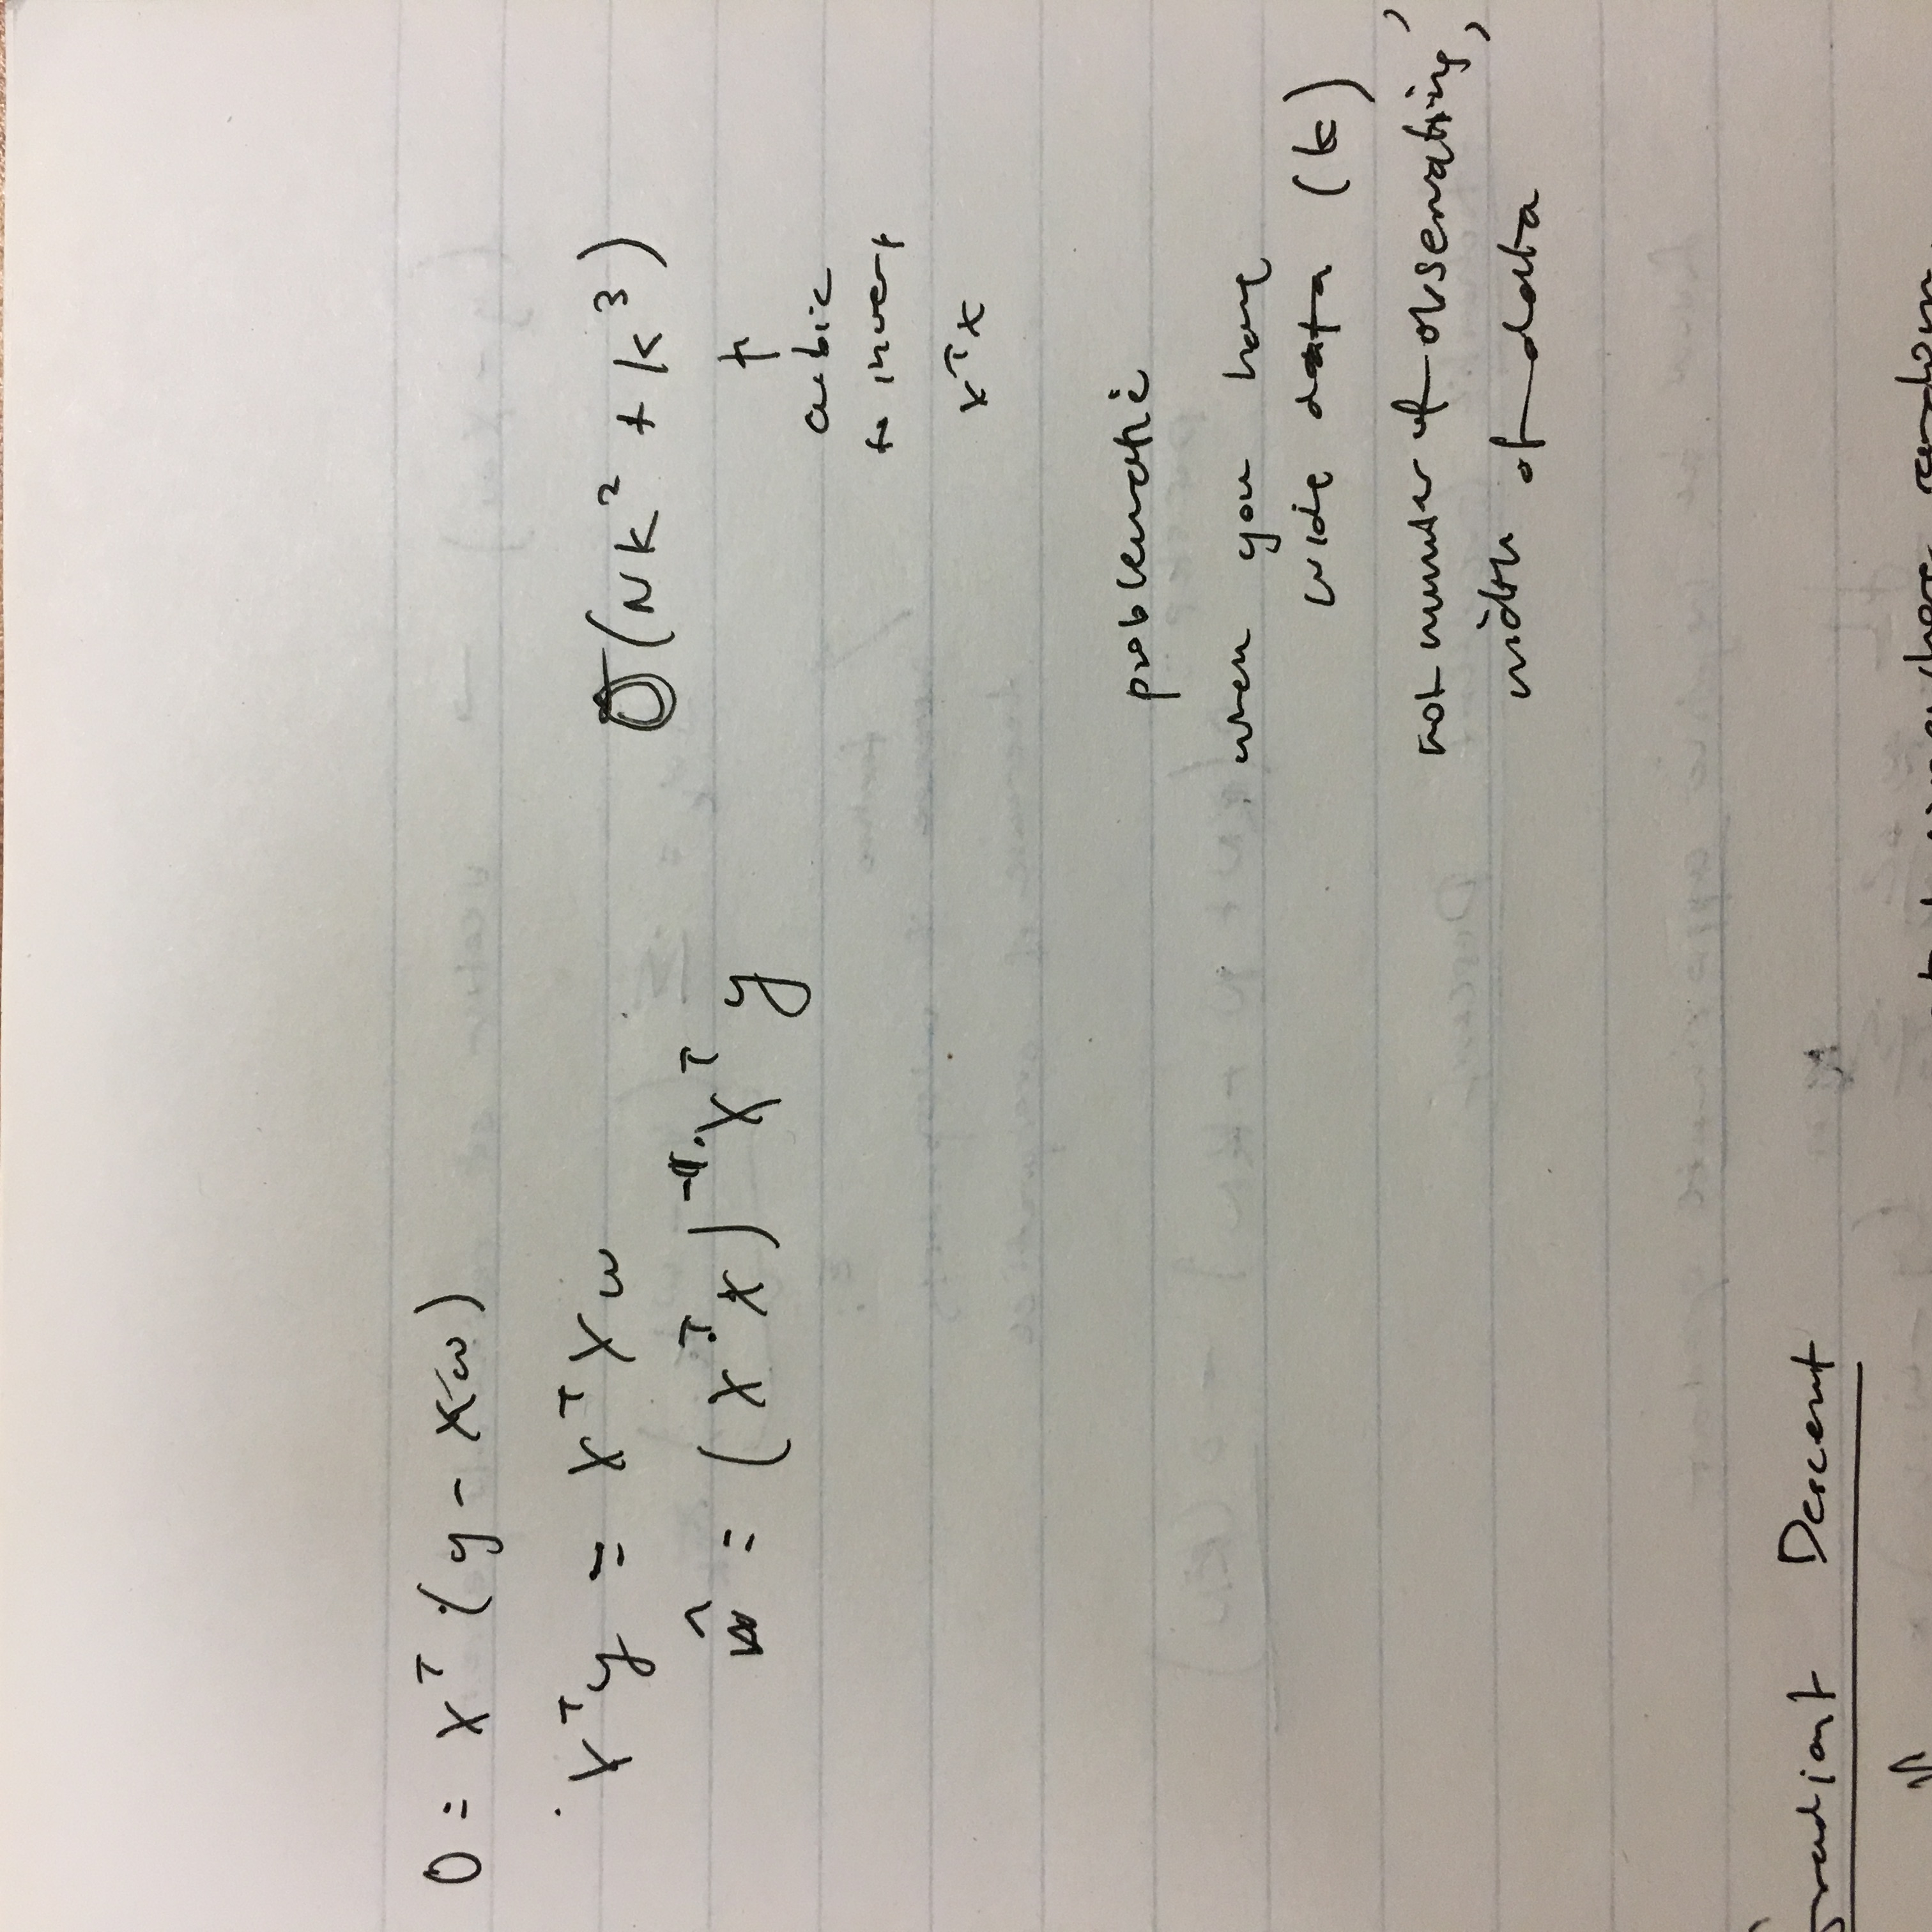
\includegraphics[width=.9\textwidth,angle=270]{figures/6.jpg}
    \caption{
      Since we are working with vectors, we can use linear algebra and matrix multiplication to solve for our coefficient vector w. Note, it becomes problematic when we have wide data (high dimensions k) as matrix operations are extremely expensive in this manner - number of observations is less impactful on runtime than width of data}
    \label{fig:example_figure8}
  \end{center}
\end{figure}

\pagebreak

Figure \ref{fig:example_figure9} Gradient Descent
\begin{figure}[ht]
  \begin{center}
    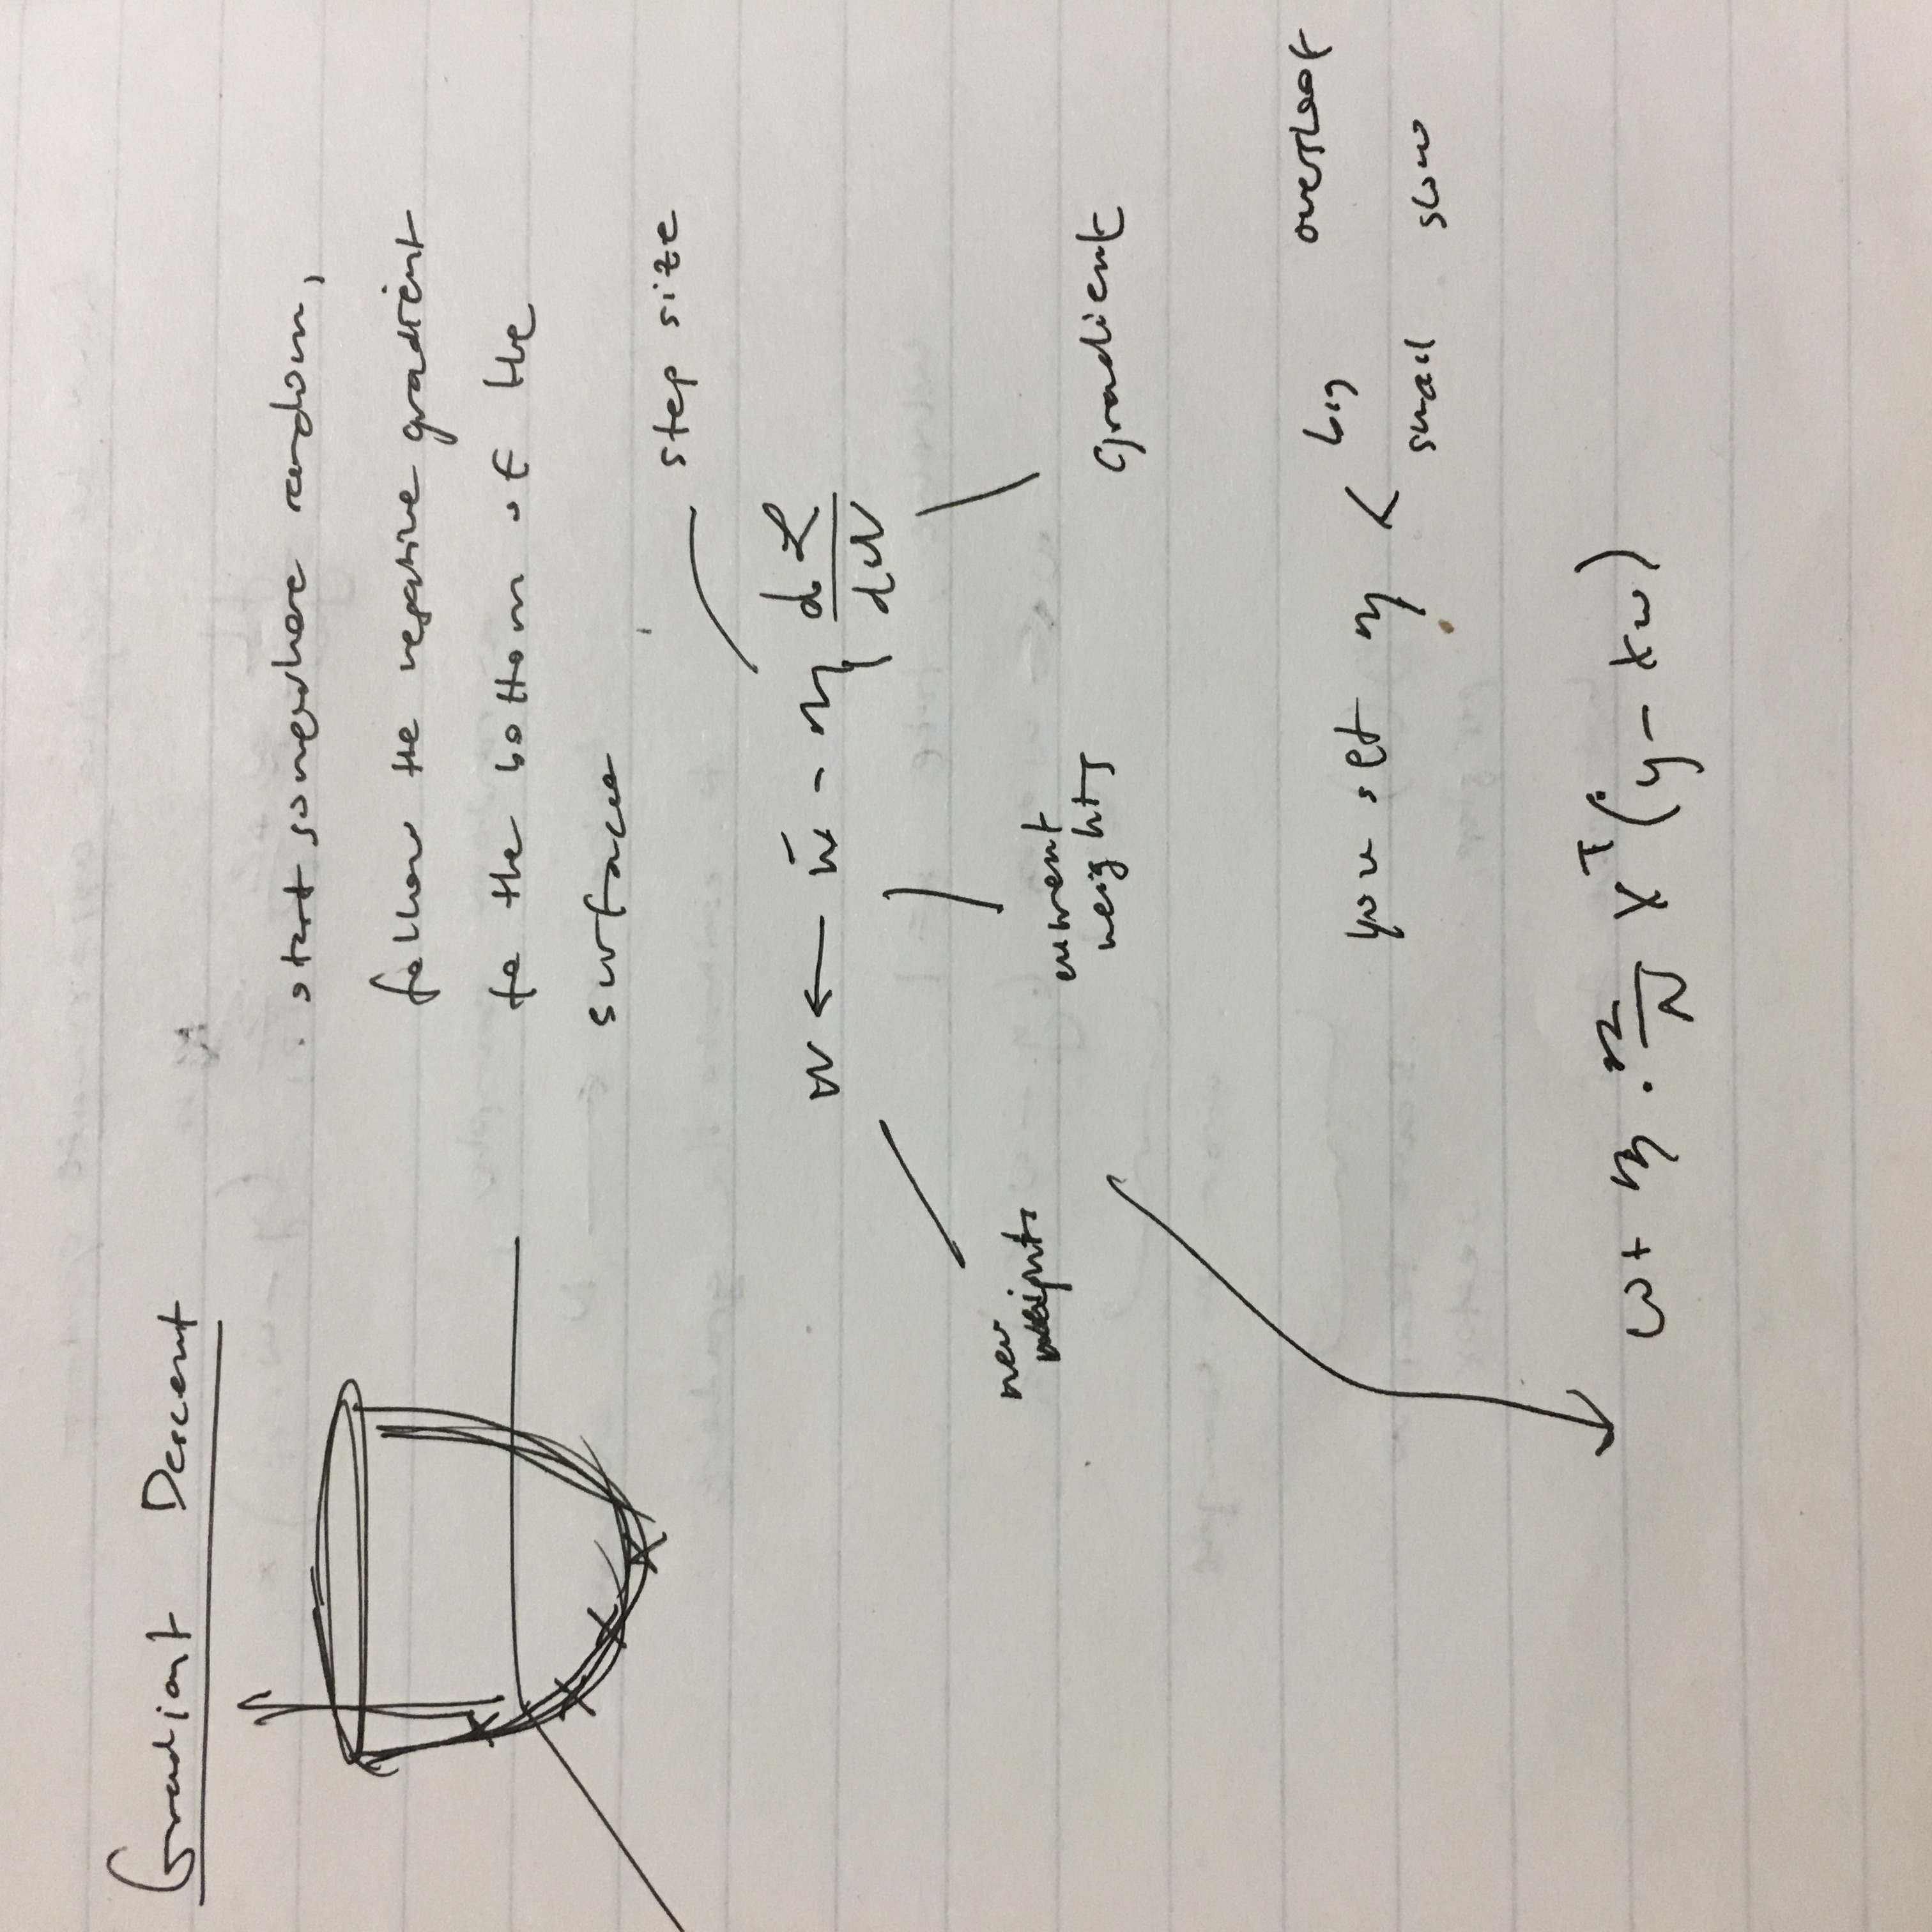
\includegraphics[width=.9\textwidth,angle=270]{figures/7.jpg}
    \caption{
      Start somewhere random, follow the negative gradient to the bottom of the surface.
      You set the learning rate (can be variable) - too big and it will overshoot the minimum, 
      too small and gradient descent will take a long time}
    \label{fig:example_figure9}
  \end{center}
\end{figure}

\pagebreak

Figure \ref{fig:example_figure10} Vector of residuals/errors
\begin{figure}[ht]
  \begin{center}
    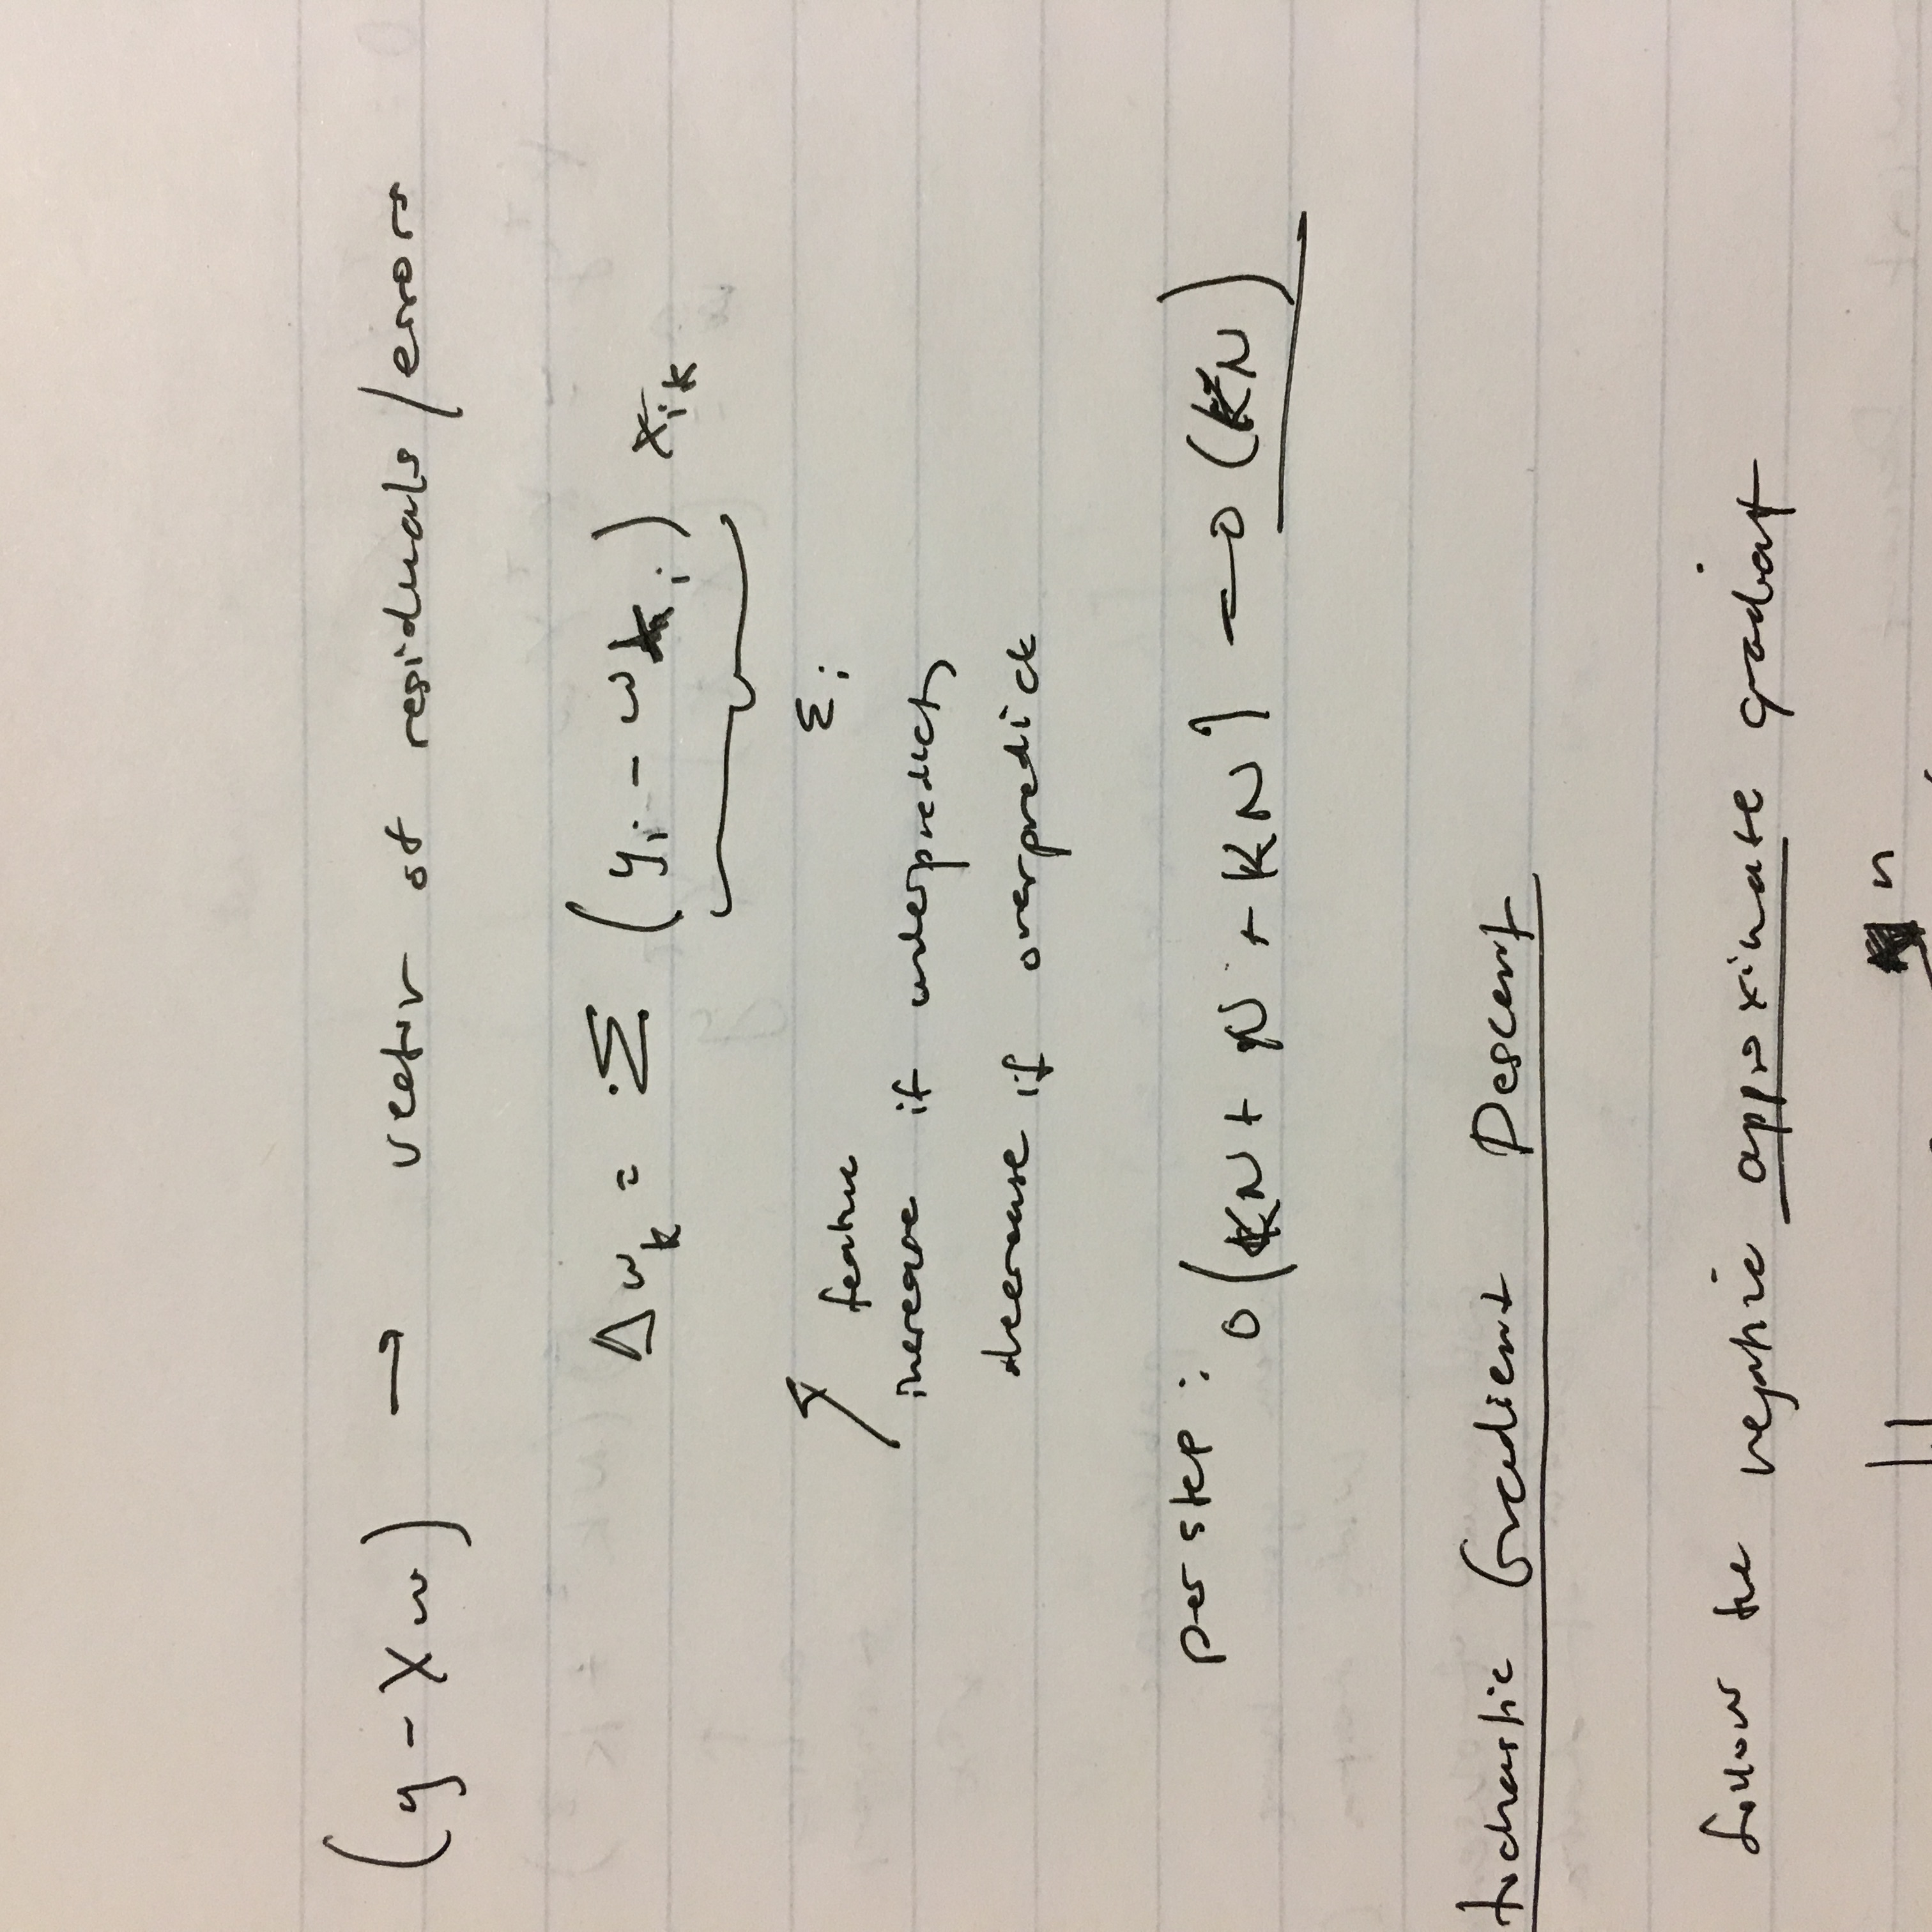
\includegraphics[width=.9\textwidth,angle=270]{figures/8.jpg}
    \caption{
      Increase features w if underpredict, decrease features w if overpredict }
    \label{fig:example_figure10}
  \end{center}
\end{figure}

\pagebreak

Figure \ref{fig:example_figure11} Stochastic Gradient Descent

\begin{figure}[ht]
  \begin{center}
    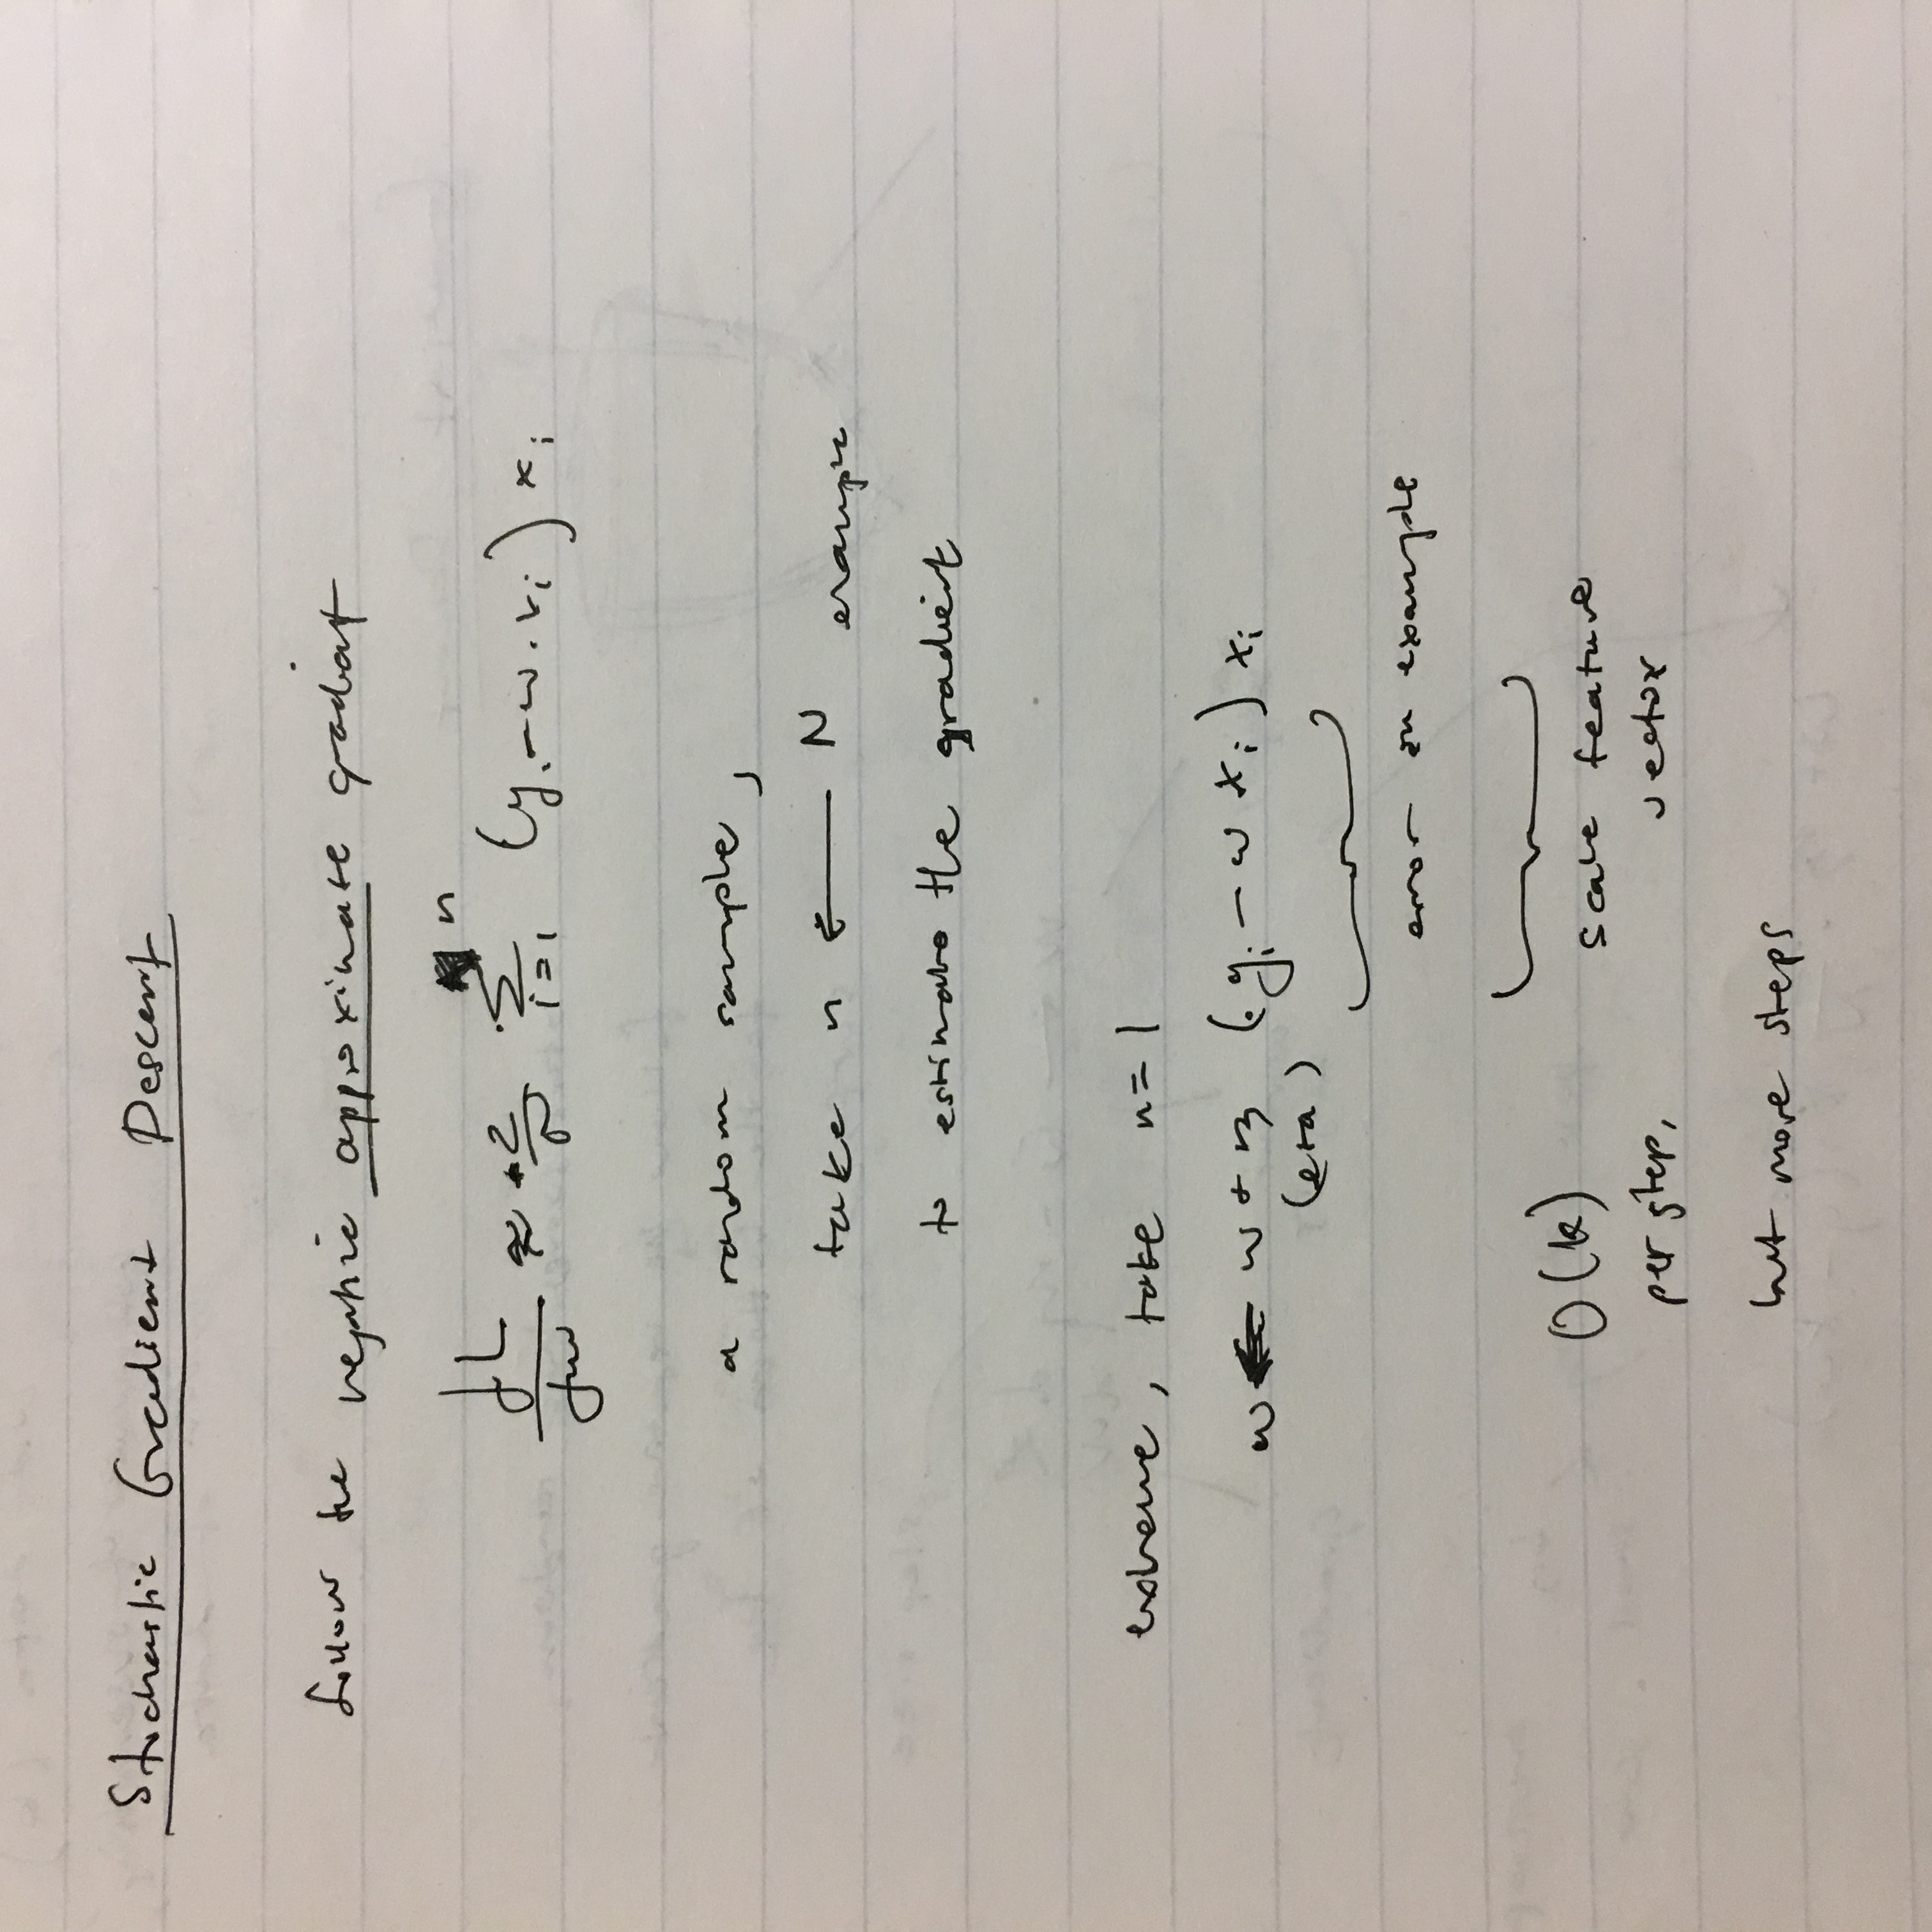
\includegraphics[width=.9\textwidth,angle=270]{figures/9.jpg}
    \caption{
      Follow the negative approximate gradient - take an n random sample to estimate the gradient}
    \label{fig:example_figure11}
  \end{center}
\end{figure}
